%%%%%%%%%%%%%%%%%%%%%%%%%%%%%%%%%%%%%%%%%%%%%%%%%%%%%%%%%%%%%%%%%%%%%%%%
\section{Meanders as random surfaces}\label{sec:surfaces}
%%%%%%%%%%%%%%%%%%%%%%%%%%%%%%%%%%%%%%%%%%%%%%%%%%%%%%%%%%%%%%%%%%%%%%%%

This section explains the physical argument behind~\eqref{eq:alpha}. Each step is either a
theorem about simpler objects or a prediction, and we say which.

\subsection{A sphere made of squares}

Turn each crossing of the river and the road into a small square tile. The river enters and
leaves the tile through two opposite sides, and the road through the other two
(Figure~\ref{fig:tile}). When two crossings are neighbors along the river, glue their tiles
along the sides through which the river passes from one to the other, and do the same for
neighbors along the road. The river is an infinite straight line; add a point at infinity, so
that the plane becomes a sphere and the river becomes a closed loop. With this, every side of
every tile is glued to a side of another tile, and the tiles form a closed surface shaped like a
sphere.

\begin{figure}[t]
\centering
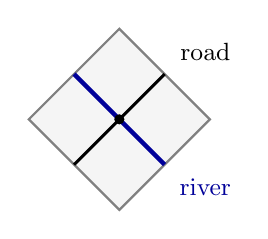
\begin{tikzpicture}[scale=1.15]
  \draw[gray,line width=0.8pt,fill=gray!8] (0,1)--(1,0)--(0,-1)--(-1,0)--cycle;
  \draw[blue!60!black,line width=1.6pt] (-0.5,0.5)--(0.5,-0.5);
  \draw[line width=1.1pt] (0.5,0.5)--(-0.5,-0.5);
  \fill (0,0) circle[radius=1.6pt];
  \node[blue!60!black,font=\small] at (0.95,-0.75) {river};
  \node[font=\small] at (0.95,0.75) {road};
\end{tikzpicture}
\caption{One crossing becomes one square tile; the river and the road each pass through it once.
Gluing the tiles of all $2n$ crossings gives a sphere made of $2n$ squares, with two curves drawn
on it that each pass through every square once.}
\label{fig:tile}
\end{figure}

So a meander of order $n$ is a sphere built from $2n$ squares, together with two curves on it,
the river and the road, each of which passes through every square exactly once. Counting
meanders means counting such decorated spheres.

\subsection{Random surfaces without drawings}

The sphere of squares can also be drawn directly from the picture of the meander, and this is
the easiest way to see what kind of object it is (Figure~\ref{fig:spheres}). The river and the
road cut the plane into regions; recall that the river is closed up through a point at infinity,
so the region above the river and the region below it at infinity are different. Put a dot in each
region. Each piece of river or road between two crossings separates two regions; join their dots
by an edge that crosses that piece. Each crossing is then surrounded by exactly four edges, so it
becomes a square, and these squares are the tiles of Figure~\ref{fig:tile}. A meander of order $n$
gives $2n+2$ dots, $4n$ edges and $2n$ squares. For the meander of order~$2$ in
Figure~\ref{fig:spheres}(a), the six regions $v_1,\ldots,v_6$ give the sphere in panel~(b): two
points $v_1$ and $v_6$ joined by four paths of length two, through $v_2$, $v_3$, $v_4$ and $v_5$,
with a square between each pair of neighboring paths (one of them is the outside of the
picture).

\begin{figure}[t]
\centering
% Spheres of squares from meanders (Section 3.2). Regions of the plane become vertices,
% pieces of river and road become edges, crossings become square faces.
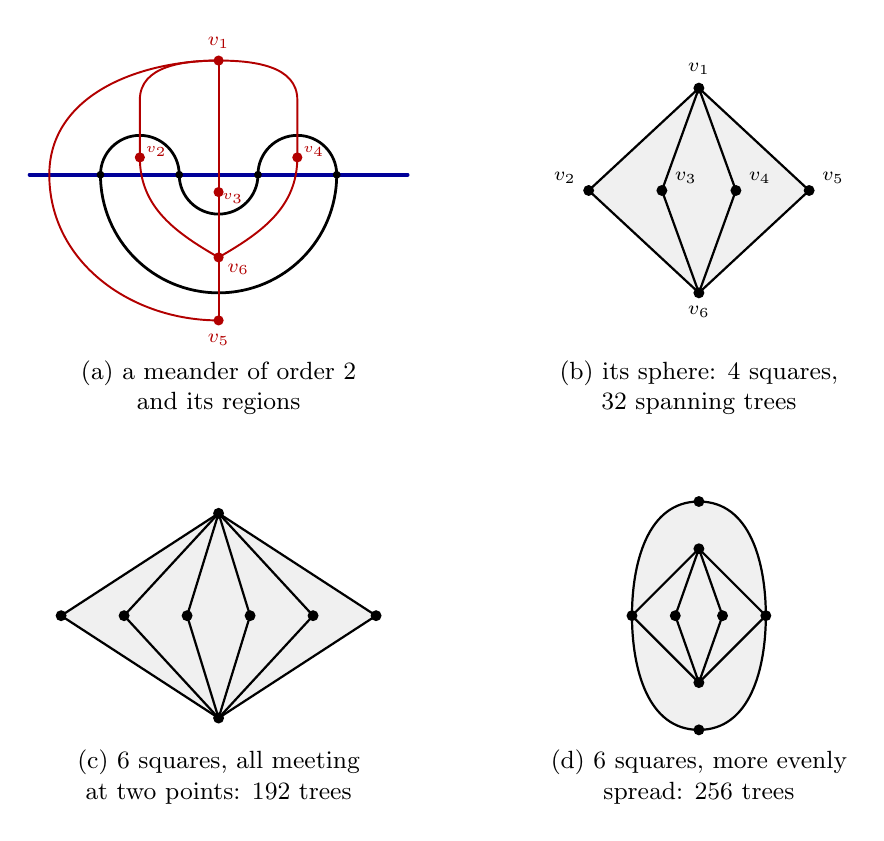
\begin{tikzpicture}[line cap=round]
  \tikzset{reg/.style={circle,fill=red!70!black,inner sep=1.3pt},
           dual/.style={red!70!black,line width=0.7pt},
           qv/.style={circle,fill=black,inner sep=1.4pt},
           qe/.style={line width=0.8pt},
           lab/.style={font=\scriptsize}}
  % ---------- (a) meander of order 2 with its regions ----------
  \begin{scope}[x=1cm,y=1cm]
    \draw[blue!60!black,line width=1.4pt] (0.1,0)--(4.9,0);
    \begin{scope}[line width=1pt]
      \draw (1,0) arc[start angle=180,end angle=0,radius=0.5];
      \draw (3,0) arc[start angle=180,end angle=0,radius=0.5];
      \draw (1,0) arc[start angle=180,end angle=360,radius=1.5];
      \draw (2,0) arc[start angle=180,end angle=360,radius=0.5];
    \end{scope}
    \foreach \k in {1,...,4} \fill (\k,0) circle[radius=1.4pt];
    % dual edges
    \draw[dual] (1.5,0.22)--(1.5,0.95) to[out=90,in=180] (2.5,1.45);
    \draw[dual] (3.5,0.22)--(3.5,0.95) to[out=90,in=0] (2.5,1.45);
    \draw[dual] (2.5,1.45)--(2.5,-0.22);
    \draw[dual] (1.5,0.22) to[out=-90,in=150] (2.5,-1.05);
    \draw[dual] (3.5,0.22) to[out=-90,in=30] (2.5,-1.05);
    \draw[dual] (2.5,-0.22)--(2.5,-1.05)--(2.5,-1.85);
    \draw[dual] (2.5,1.45) to[out=180,in=90] (0.35,0) to[out=-90,in=180] (2.5,-1.85);
    \foreach \p/\n/\a in {(1.5,0.22)/A/north,(3.5,0.22)/B/north,(2.5,1.45)/U/south,(2.5,-0.22)/C/east,(2.5,-1.05)/D/east,(2.5,-1.85)/L/north} {
      \node[reg] at \p {}; }
    \node[lab,font=\tiny,red!70!black] at (1.71,0.29) {$v_2$};
    \node[lab,font=\tiny,red!70!black] at (3.71,0.29) {$v_4$};
    \node[lab,red!70!black] at (2.5,1.68) {$v_1$};
    \node[lab,font=\tiny,red!70!black] at (2.68,-0.30) {$v_3$};
    \node[lab,red!70!black] at (2.75,-1.2) {$v_6$};
    \node[lab,red!70!black] at (2.5,-2.1) {$v_5$};
    \node[font=\small,align=center] at (2.5,-2.7) {(a) a meander of order $2$\\ and its regions};
  \end{scope}
  % ---------- (b) its sphere: four squares ----------
  \begin{scope}[xshift=8.6cm,yshift=-0.2cm]
    \fill[gray!12] (0,1.3)--(-1.4,0)--(0,-1.3)--(1.4,0)--cycle;
    \foreach \x/\n/\dx/\an in {-1.4/2/-0.04/east,-0.47/3/0.04/west,0.47/4/0.04/west,1.4/5/0.04/west} {
      \draw[qe] (0,1.3)--(\x,0)--(0,-1.3);
      \node[qv] at (\x,0) {}; \node[lab,anchor=\an] at (\x+\dx,0.16) {$v_\n$};}
    \node[qv] at (0,1.3) {}; \node[lab,anchor=south] at (0,1.35) {$v_1$};
    \node[qv] at (0,-1.3) {}; \node[lab,anchor=north] at (0,-1.35) {$v_6$};
    \node[font=\small,align=center] at (0,-2.5) {(b) its sphere: $4$ squares,\\ $32$ spanning trees};
  \end{scope}
  % ---------- (c) the six-square sphere where all squares meet at two points ----------
  \begin{scope}[yshift=-5.6cm,xshift=2.5cm]
    \fill[gray!12] (0,1.3)--(-2.0,0)--(0,-1.3)--(2.0,0)--cycle;
    \foreach \x in {-2.0,-1.2,-0.4,0.4,1.2,2.0} {
      \draw[qe] (0,1.3)--(\x,0)--(0,-1.3); \node[qv] at (\x,0) {};}
    \node[qv] at (0,1.3) {}; \node[qv] at (0,-1.3) {};
    \node[font=\small,align=center] at (0,-2.05) {(c) $6$ squares, all meeting\\ at two points: $192$ trees};
  \end{scope}
  % ---------- (d) the six-square sphere of the meander of Figure 1 ----------
  \begin{scope}[yshift=-5.6cm,xshift=8.6cm]
    \coordinate (U) at (0,0.85); \coordinate (C) at (0.85,0); \coordinate (G) at (0,-0.85); \coordinate (E) at (-0.85,0);
    \fill[gray!12] (C) to[out=90,in=0] (0,1.45) to[out=180,in=90] (E) to[out=-90,in=180] (0,-1.45) to[out=0,in=-90] (C);
    \draw[qe] (U)--(C)--(G)--(E)--cycle;
    \draw[qe] (U)--(-0.3,0)--(G);
    \draw[qe] (U)--(0.3,0)--(G);
    \draw[qe] (C) to[out=90,in=0] (0,1.45) to[out=180,in=90] (E);
    \draw[qe] (C) to[out=-90,in=0] (0,-1.45) to[out=180,in=-90] (E);
    \foreach \p in {(U),(C),(G),(E),(0,1.45),(0,-1.45),(-0.3,0),(0.3,0)} \node[qv] at \p {};
    \node[font=\small,align=center] at (0,-2.05) {(d) $6$ squares, more evenly\\ spread: $256$ trees};
  \end{scope}
\end{tikzpicture}

\caption{From a meander to a sphere of squares. (a) The meander of order $2$ whose upper arches
join $1$--$2$ and $3$--$4$ and whose lower arches join $1$--$4$ and $2$--$3$. Each region gets a
dot, and each piece of river or road becomes an edge (red) between the dots on its two sides.
(b) The resulting sphere, redrawn: each crossing has become a square, and the outside of the
picture is the fourth square. (c), (d) Two spheres of six squares that come from meanders of
order $3$; (d) comes from the meander of Figure~\ref{fig:meander}. They carry $192$ and $256$
spanning trees.}
\label{fig:spheres}
\end{figure}

A graph drawn on the sphere without crossings, considered up to deformation, is called a
\emph{planar map}. Its \emph{faces} are the regions into which the edges cut the sphere, and a
sphere glued from squares is a planar map in which every face has four sides. Not every such
sphere comes from a meander, since a meander also carries the river and the road, but every
sphere of squares is a random-surface model in its own right. Such spheres, with nothing drawn on
them, are well understood. Tutte counted them in the 1960s~\cite{Tutte}: with one marked edge
(which removes symmetries), the numbers with $1,2,3,4,5$ squares are $2, 9, 54, 378, 2916$, and
with $n$ squares there are about
\[ 12^n\, n^{-5/2} \]
of them. Here $n$ counts squares, while a meander of order $n$ has $2n$ squares; the exponent
does not depend on this choice of scale. Glued from triangles instead, the count grows at a
different rate but with the same power $n^{-5/2}$. This is universality again, now for surfaces.
Zoomed out, a uniformly random sphere glued from many squares, or from many triangles, looks like
one and the same random surface, called the \emph{Brownian map}; it plays the role that Brownian
motion plays for walks~\cite{LeGall,Miermont}.

In physics, a sum over random geometries of space is called a theory of \emph{quantum gravity}.
In two dimensions a geometry is just a surface, so ``two-dimensional quantum gravity'' means
nothing more than a random surface. No actual gravity is involved, and the name is used below
only when quoting the physics literature.

\subsection{One drawing: a spanning tree}

Now draw something on the surface and count surfaces together with drawings. The simplest case
is a \emph{spanning tree}: a set of edges that connects every vertex without closing any loop.
Mullin showed that the planar maps with $n$ edges and a marked spanning tree number exactly
$\mathrm{Cat}_n\mathrm{Cat}_{n+1}$~\cite{Mullin}, so about
\[ 16^n\, n^{-3} \]
up to a constant factor (again with one marked edge). The exponent has moved from $5/2$ to $3$.
The proof explains why. A map with a spanning tree can be read as two interleaved bracket words,
one for the tree and one for the edges outside it; a \emph{bracket word} is a sequence of opening
and closing brackets that match up, like the arch systems above. Each word is a walk that comes
back and stays above its start, so the exponent is $3/2+3/2$.

A meander carries two drawings, the river and the road. Each is a single curve that visits
every square once. Physicists expect such a curve to constrain the surface, at large scales, in
the same way as a spanning tree: both are ``space filling'' in the sense that they reach every
part of the surface, and in the zoomed-out limit both become the same kind of random curve. If
this is right, a meander is a random surface with two tree-like drawings, and its exponent
should be the next step up from~$3$.

\subsection{The effect of a drawing on the surface}\label{sec:charge}

Counting surfaces with drawings means summing, over all surfaces, the number of drawings each
one can carry. A surface that can carry many drawings is counted many times, so the drawing
changes which surfaces are typical.

Figure~\ref{fig:spheres} shows this at six squares. Sphere~(c) carries $192$ spanning trees and
sphere~(d) carries $256$, so when surfaces are counted together with their spanning trees, (d)
counts $4/3$ times as much as~(c). In~(c) all six squares meet at the same two points; in~(d)
they are spread more evenly. The same pattern holds at eight squares: the $42$ meanders of
order~$4$ give spheres carrying between $1024$ and $2048$ spanning trees, the fewest when all
squares meet at two points and the most when the squares are spread most evenly.

The reason is a \emph{neck}: a short closed curve on the surface that separates it into two large
pieces. A tree has to cross a neck through its few edges, so the parts of the tree on the two
sides are almost independent, and many combinations that a round surface would allow are lost.
Intuitively, trees prefer round, well-connected surfaces and penalize thin necks. A curve that
must visit every square behaves the same way, since it too has to pass back and forth through any
neck.

How strongly a drawing does this is measured by a single number $c$, which physicists call the
\emph{central charge} of the drawing. It can be described by counting alone. The number of
spanning trees of a graph is a determinant, by Kirchhoff's theorem: write $\det\Delta_G$ for the
determinant of the \emph{Laplacian matrix} of the surface $G$ with one row and column removed.
(The Laplacian matrix of a graph has the vertex degrees on its diagonal and, off the diagonal,
minus the number of edges between the two vertices.) This determinant is large for round,
well-connected surfaces and small for pinched ones. For many kinds of drawings, the number of
drawings that a large surface $G$ can carry is predicted to behave like
\begin{equation}\label{eq:charge}
\#\{\text{drawings on } G\} \;\approx\; \rho^{|G|}\,\big(\det\Delta_G\big)^{-c/2},
\end{equation}
where $|G|$ is the number of squares, $\rho$ is a constant that depends on the kind of drawing but
not on the surface, and the second factor carries all the dependence on the shape of $G$. The
exponent in~\eqref{eq:charge} defines $c$.
\begin{itemize}
\item \emph{Nothing drawn.} Every surface carries exactly one empty drawing, so $c=0$.
\item \emph{A spanning tree.} The number is exactly $\det\Delta_G$, so $c=-2$.
\item \emph{Two independent drawings.} Their numbers multiply, so the powers of the determinant
add, and so do the values of $c$. Two spanning trees give $(\det\Delta_G)^2$, that is, $c=-4$.
\item \emph{A random height at each vertex}, with a Gaussian weight that penalizes differences
between neighbors (the discrete Gaussian free field). Its total weight is proportional to
$(\det\Delta_G)^{-1/2}$, so $c=+1$. Positive $c$ favors pinched surfaces.
\item \emph{A single curve that visits every square once}, like the river or the road. Its number
is not a determinant. Physicists predict that at large scales it behaves as if $c=-2$, like a
spanning tree: both reach every part of the surface, and in the zoomed-out limit both become the
same kind of random curve. A meander, with two such curves, is therefore predicted to have
$c=-2+(-2)=-4$.
\end{itemize}
So negative $c$ means a preference for round surfaces with few thin necks, and the more negative
$c$ is, the stronger the preference. For trees, \eqref{eq:charge} is an identity; for the curves of
a meander it is the first of the two unproved assumptions of the physical argument.

\subsection{The KPZ formula}

A rule found in physics, the Knizhnik--Polyakov--Zamolodchikov (KPZ) formula~\cite{KPZ}, turns
$c$ into the counting exponent. Applied to meanders by Di~Francesco, Golinelli and
Guitter~\cite{DGG}, it reads
\begin{equation}\label{eq:kpz}
\alpha \;=\; 1+x, \qquad x+\frac1x \;=\; \frac{13-c}{6},\quad x\ge1.
\end{equation}
Here $x$ is the larger of the two roots of the quadratic equation. It has its own meaning: if
surfaces of size exactly $n$ are counted with weight about $n^{-\alpha}$, then the total weight of
sizes at least $n$ is about $n^{-(\alpha-1)}=n^{-x}$, so $x$ is the exponent of this \emph{tail}.
Section~\ref{sec:continuum} describes a model in which the formula is proved, in Paper~D, by
computing exactly such a tail.
At $c=0$ it gives $x=3/2$ and $\alpha=5/2$, Tutte's exponent. At $c=-2$ it gives $x=2$ and
$\alpha=3$, Mullin's exponent. At $c=-4$ the equation $x+1/x=17/6$ becomes $6x^2-17x+6=0$, so
$x=(17+\sqrt{145})/12$ and
\[ \alpha \;=\; \frac{29+\sqrt{145}}{12}\;\approx\;3.4201 .\]
The square root appears because~\eqref{eq:kpz} is a quadratic equation for $x$. The rule does
not add up exponents. It adds up central charges and then solves for $\alpha$.

\begin{figure}[t]
\centering
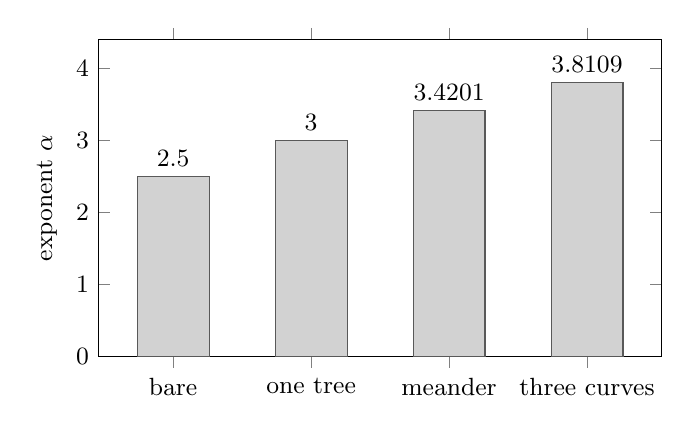
\begin{tikzpicture}
\begin{axis}[ybar,width=0.72\textwidth,height=5.6cm,ymin=0,ymax=4.4,bar width=26pt,
  symbolic x coords={bare,one tree,meander,three curves},xtick=data,
  nodes near coords,nodes near coords style={font=\small},
  every node near coord/.append style={/pgf/number format/fixed,/pgf/number format/precision=4},
  ylabel={exponent $\alpha$},tick label style={font=\small},label style={font=\small},
  enlarge x limits=0.18]
\addplot[fill=gray!35,draw=gray!70!black] coordinates {(bare,2.5) (one tree,3) (meander,3.4201) (three curves,3.8109)};
\end{axis}
\end{tikzpicture}
\caption{The exponent from~\eqref{eq:kpz} for a bare surface ($c=0$), one tree ($c=-2$), two
tree-like curves as in a meander ($c=-4$), and three ($c=-6$). The steps shrink: $+0.5$,
$+0.42$, $+0.39$.}
\label{fig:staircase}
\end{figure}

Figure~\ref{fig:staircase} shows the effect. If the two drawings of a meander simply added their
effects, each would raise the exponent by $1/2$ and meanders would have $\alpha=3.5$. The steps
shrink instead. Intuitively, both drawings live on the same surface, and each additional drawing
has less effect on a surface that the others have already made round.

The first two values of~\eqref{eq:kpz} agree with theorems of Tutte and Mullin. The third, for
meanders, rests on two assumptions that have not been proved for meanders: that each curve
counts as $c=-2$, and that the two curves are independent enough at large scales for their
central charges to add.

\subsection{The exponent and the shape of the surface}\label{sec:shape}

The exponent also has a direct geometric meaning in terms of necks. Take a meander of order $2m$
and draw a vertical line through the middle of the river, between crossings $2m$ and $2m+1$.
Suppose the road meets this line only twice, both times above the river. On the sphere of squares
the line is then a neck that crosses the drawing only twice, and cutting along it and reconnecting
the two road ends on each side produces two meanders of order $m$. Call an arch above the river
\emph{outermost} if no other arch above the river passes over it. The cut-off piece on each side
carries a marked outermost arch, the one created by the reconnection, and conversely two meanders
of order $m$, each with one marked outermost arch, can be glued back in exactly one way. A meander
has at least one outermost arch above the river and, on average, a bounded number of them
(Paper~C). So the number of such meanders lies between $M_m^2$ and a constant times $M_m^2$, and
the chance that a random meander of order $2m$ has this thin neck at its middle is, up to
constant factors,
\[ \frac{M_m^2}{M_{2m}} \;\approx\; \frac{(A\mu^m m^{-\alpha})^2}{A\mu^{2m}(2m)^{-\alpha}} \;=\; A\,2^{\alpha}\, m^{-\alpha} .\]
Here we used the law~\eqref{eq:law}. So $\alpha$ is the exponent of the probability of a thin
neck that cuts the surface into two equal halves. For walks that stay above their start, the same calculation with
Catalan numbers gives $\mathrm{Cat}_m^2/\mathrm{Cat}_{2m}\approx m^{-3/2}$: a walk returns to its starting level at its
midpoint with probability of order $m^{-3/2}$.

\begin{figure}[b]
\centering
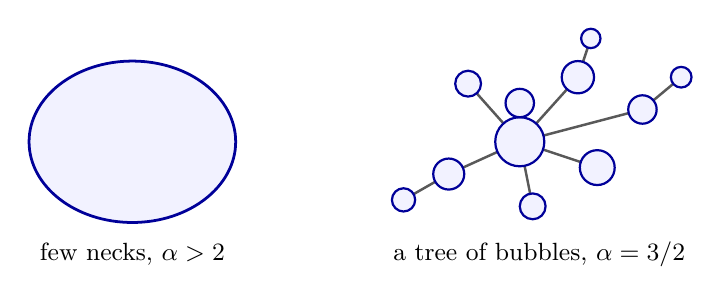
\begin{tikzpicture}[scale=0.82]
  \draw[blue!60!black,line width=1pt,fill=blue!5] (0,0) ellipse (1.6 and 1.25);
  \node[font=\small] at (0,-1.75) {few necks, $\alpha>2$};
  \begin{scope}[xshift=6cm]
  \foreach \a/\b in {0/0.6, 0.9/1.0, -0.8/0.9, 1.2/-0.4, -1.1/-0.5, 0.2/-1.0, 1.9/0.5}
     {\draw[gray!70!black,line width=0.9pt] (0,0)--(\a,\b);}
  \draw[gray!70!black,line width=0.9pt] (1.9,0.5)--(2.5,1.0) (-1.1,-0.5)--(-1.8,-0.9) (0.9,1.0)--(1.1,1.6);
  \foreach \a/\b/\r in {0/0/0.38, 0/0.6/0.22, 0.9/1.0/0.25, -0.8/0.9/0.2, 1.2/-0.4/0.27, -1.1/-0.5/0.24, 0.2/-1.0/0.2, 1.9/0.5/0.22, 2.5/1.0/0.16, -1.8/-0.9/0.18, 1.1/1.6/0.15}
     {\draw[blue!60!black,line width=0.8pt,fill=blue!5] (\a,\b) circle[radius=\r];}
  \node[font=\small] at (0.3,-1.75) {a tree of bubbles, $\alpha=3/2$};
  \end{scope}
\end{tikzpicture}
\caption{Two kinds of large random surface. Left: a round surface in which thin necks are rare.
Right: a surface that has fallen apart into small bubbles joined at necks.}
\label{fig:bubbles}
\end{figure}

Physics gives a picture of two regimes.
\begin{itemize}
\item The KPZ formula~\eqref{eq:kpz} always gives $x\ge1$, so $\alpha\ge2$. As $c$ rises to $1$
it gives $\alpha=2$, and for $c>1$ it has no real solution $x\ge1$. Wherever the formula applies,
balanced necks are rare, and a large random surface is a genuinely two-dimensional blob.
\item When the drawings make necks cheap enough, for instance when many small loops are favored
as in the next paragraph, the formula stops applying. A large random
surface then falls apart into a tree of small bubbles joined at necks
(Figure~\ref{fig:bubbles}), and the exponent is $3/2$, the exponent of trees, because the
bubbles are arranged like the vertices of a random tree.
\end{itemize}
In the physics literature a piece of surface cut off by a neck is called a \emph{baby universe}.

Meanders are predicted to sit in the first regime, but a related family crosses between the two.
A \emph{meandric system} of order $n$ is a pair of arch systems on the same $2n$ crossings, one
above and one below the river, whose arches may form any number of closed loops; meanders are the
systems with one loop. Give each system the weight $q^{k}$, where $q>0$ and $k$ is its number of
loops, and let $Z_n(q)$ be the total weight of the systems of order $n$. For $0\le q\le 2$ the
physical prediction for the exponent of $Z_n(q)$ is again of the form~\eqref{eq:kpz}, with a
central charge that depends on $q$: writing $q=2\cos(\pi\eta)$ with $0\le \eta\le 1/2$,
\[ c(q) \;=\; -1-\frac{6\eta^2}{1-\eta}, \]
which is $-1$ at $q=2$ and $-4$ at $q=0$. The value $q=0$ stands for meanders: as $q\to0$, the
weight divided by $q$ concentrates on the systems with one loop. For large $q$,
systems with many small loops win: the road is broken into many small circles, the surface
becomes a tree of small bubbles held together by the river, and the exponent drops to $3/2$. A
proof of this second regime for $q\ge 167.6$ is in the project repository~\cite{Repo}
(Appendix~\ref{app:repo}); it has not yet been independently checked, and it is not part of
Papers~B--D. Finite-size numerical measurements suggest a crossover, but do not determine the location of a
transition. Beyond $q=2$, the exponent and the onset of the tree regime remain unresolved outside the proved range.
